%% PODSTAWOWE USTAWIENIA DOKUMENTU
\documentclass[12pt, a4paper, polish]{article}
%\usepackage[a4paper, lmargin=2.5cm, rmargin=2.5cm, hmargin=2.5cm, bmargin=2.5cm]{geometry}
\usepackage[a4paper,top=2cm,bottom=2cm,left=1cm,right=1cm]{geometry}
%\geometry{verbose,lmargin=2.5cm,rmargin=2.5cm}
\usepackage{enumerate}
% Symbole matematyczne
\usepackage{latexsym}
% Formatowanie czcionki
\usepackage[T1]{fontenc}
% Formatowanie polskich znaków
\usepackage{polski}
\usepackage[utf8]{inputenc}
% Akapit po sekcji
%\usepackage{indentfirst}
% Ustawienie nagłówków i stopek
\usepackage{fancyhdr}
% Liczba stron
%\usepackage{lastpage}
% Kolumny
%\usepackage{paracol}
% Czcionka latin modern
\usepackage{lmodern}
% Równania matematyczne
\usepackage{amsmath}
\usepackage{amsfonts}
\usepackage{amssymb}
\usepackage{amsthm}
% Wstawianie grafik
\usepackage{graphicx}
\usepackage[section]{placeins} % Ogarnięcie obrazków
\usepackage{float}
\usepackage{subcaption}
%\usepackage[outdir=./]{epstopdf}
\usepackage{grffile}
\usepackage{gensymb}
\usepackage{tabularx, multirow}


%% ODSTĘPY W WIERSZACH
\setlength{\parindent}{1cm}
\setlength{\parskip}{0.01cm}
\linespread{1}

%% SZARE TŁO TEKSTU
%\usepackage[most]{tcolorbox}
%\tcbset{
%	frame code={}
%	center title,
%	left=0pt,
%	right=0pt,
%	top=0pt,
%	bottom=0pt,
%	colback=gray!30,
%	colframe=white,
%	width=\dimexpr\textwidth\relax,
%	enlarge left by=0mm,
%	boxsep=5pt,
%	arc=0pt,outer arc=0pt,
%}

% HIPERŁĄCZA SPISU TREŚCI
\usepackage{hyperref}
\hypersetup{
	colorlinks,
	citecolor=black,
	filecolor=black,
	linkcolor=black,
	urlcolor=black
}

\begin{document}
	\fancyhf{}	% Usunięcie domyślnego stylu numerowania
	
	% ********************** TYTUŁ ****************************
	\noindent\textsf{\begin{Large}Laboratorium Sterowania Robotów Mobilnych\\\end{Large}
		Raport\\
		Szymon Kacperek, Tomasz Smaruj \\
		AiR, studia stacjonarne II stopnia,  specjalność SSiR, rok akademicki 2020/2021\\
		\rule{\columnwidth}{0.2pt}}
	
	\thispagestyle{empty}
	\pagestyle{fancy}
	\fancyhead{}
	\rhead{\thepage}
	\renewcommand{\headrulewidth}{0pt}%{}
	\setlength{\footskip}{1mm}
	
	%							*****************POCZĄTEK DOKUMENTU*****************
	\tableofcontents
\newpage\section{Wstęp}
Celem omawianych ćwiczeń laboratoryjnych było zapoznanie się oraz zrozumienie zagadnień z zakresu sterowania robotów mobilnych. W kolejnych ćwiczeniach wykonywane zostały poszczególne etapy pracy - od tworzenia modelu robota do projektowania sterownika. Efektem końcowym miało być zamodelowanie układu sterowania robota mobilnego o ograniczonej mobilności z kinematyką (2,0).  Do realizacji tego zadania użyty został skrypt „Sterowanie robotów mobilnych – laboratorium (Maciej Michałek, Dariusz Pazderski)”. 

Poruszanie się robota, jest zależne od postawionych przed nim zadań ruchu. W ćwiczeniu badano trzy podstawowe zadania ruchu dla robota mobilnego:
\begin{itemize}
	\item ZD1: Zadanie śledzenia trajektorii
	\item ZD2: Zadanie sterowania do punktu
	\item ZD3: Zadanie podążania według ścieżki
\end{itemize}



\indent Do zrealizowania zadań sterowania zostały użyte trzy typy sterowników, wynikające z różnych interpretacji matematycznych. Są to następująco:
\begin{itemize}
	\item S1. Sterowniki wynikające z technik linearyzacji – dla wszystkich trzech zadań ruchu. 
	\item S2. Ciągły stabilizator Pometa jawnie zależny od czasu – tylko dla zadania stabilizacji w punkcie
	\item S3. Sterowniki nieciągłe metody VFO – dla wszystkich zadań ruchu.
\end{itemize}
\section{Krótkie omówienie poszczególnych zadań sterowania i metod sterowania}
\subsection{Sterowniki wynikające z technik linearyzacji}
Jako, że robot mobilny należy do układów nieliniowych, to sterowanie takiego robota jest trudniejsze, niż w przypadku układów liniowych. Dlatego sterowniki wynikające z tej metody polegają na dodaniu do układu linearyzującego sprzężenia zwrotnego od stanu. Linearyzację można wykonać przez dwa postępowania:\\
• Wyznaczanie liniowej aproksymacji wynikającej z rozwinięcia w szereg Taylora w pobliżu pewnego punktu pracy. \\
• Poprzez przekształcenie w torze wejście-wyjście zmiennych stanu oraz wejść sterujących korzystając ze sprzężenia zwrotnego.\\
Sterownik ten sprawdzi się do śledzenia trajektorii, odtwarzania pozycji oraz podążania wzdłuż ścieżki. 
\subsection{Ciągły stabilizator Pometa jawnie zależny od czasu}
Metoda ta przeznaczona jest dla zadania stabilizacji w punkcie. Głównym problemem dojazdu do punktu jest brak ustawicznego pobudzenia, jak np. w przypadku zadania śledzenia trajektorii, gdzie jest ona zależna od czasu. Dla zadania dojazdu do punktu jest on niezmienny w czasie.  
Główną koncepcją tego sterowania jest to, aby zastąpić pubudzenie pochodzące od generatora sygnałów referencyjnych pobudzeniem sztucznie generowanym w sprzężeniu zwrotnym. Wykorzystana do tego zostanie funkcja zależna od czasu, która pozwoli ominąć ograniczenia wynikające z twierdzenia Broketta i ustawicznie pobudzać docelowy punkt.
\subsection{Sterowniki nieciągłe metody VFO}
Metoda VFO bazuje na orientowaniu pól wektorowych, rozwiązując zadania śledzenia trajektorii zmiennych w czasie oraz dojazd do punktu. Wektorowe pole zbieżności:
$$
h(q,\ldotp)=\begin{bmatrix}h_\theta(q,\ldotp) \\ h_x(q,.) \\ h_y(q,.)\end{bmatrix}=\begin{bmatrix}h_\theta(q, .) \\ \bar{h}(q,.) \end{bmatrix}\in \rm I\!R
$$

\section{Prezentacja wyników}
\subsection{Sterowniki wynikające z technik linearyzacji}\label{linear_ps}
\subsubsection{Algorytm dla zadania odtwarzania pozycji}\label{linear_tt}
\begin{figure}[H]
	a)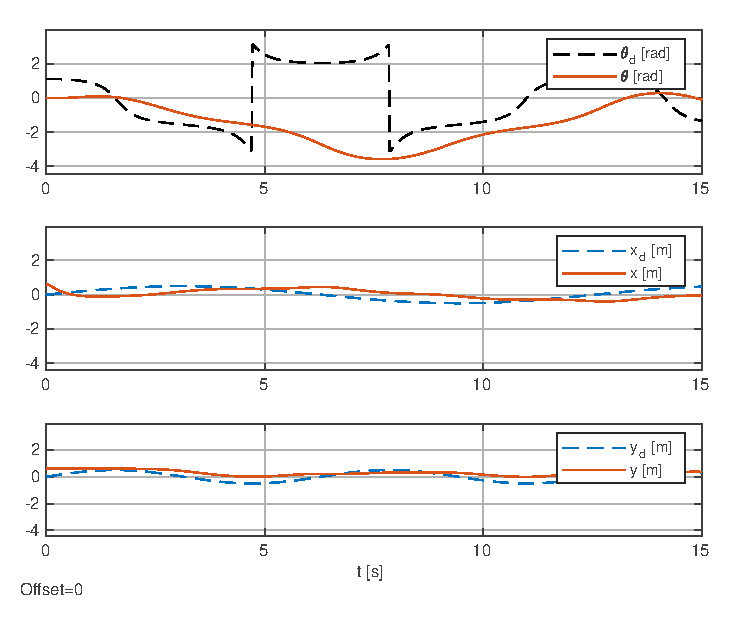
\includegraphics[width=0.5\linewidth]{lin/feedback/q.eps}
	b)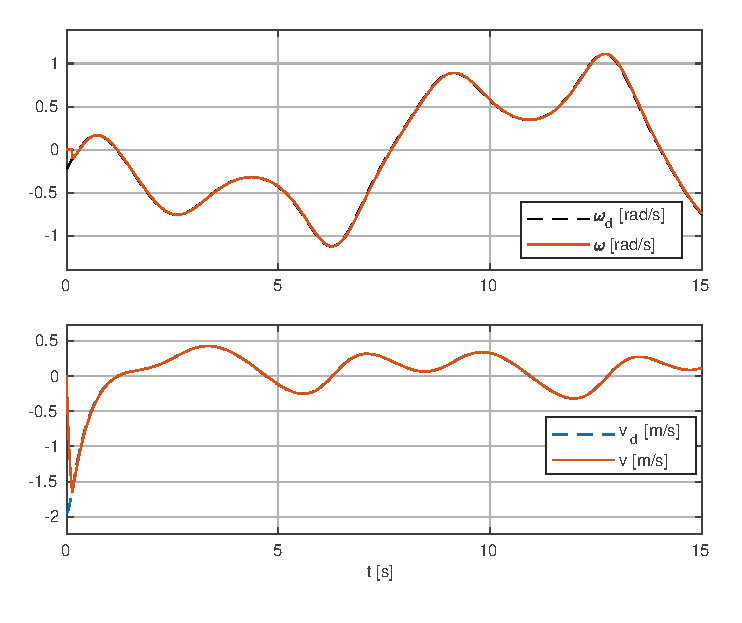
\includegraphics[width=0.5\linewidth]{lin/feedback/u.eps}\\
	c)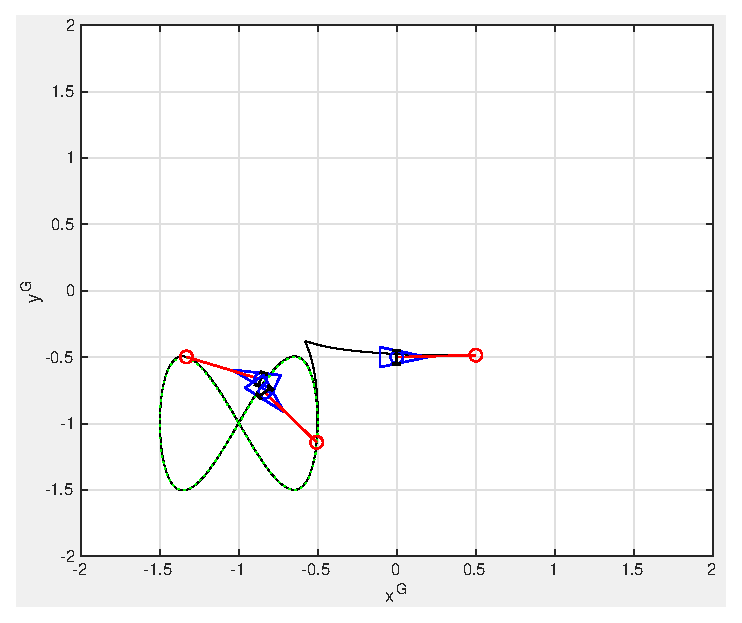
\includegraphics[width=0.5\linewidth]{lin/feedback/cartplot.eps}	
	d)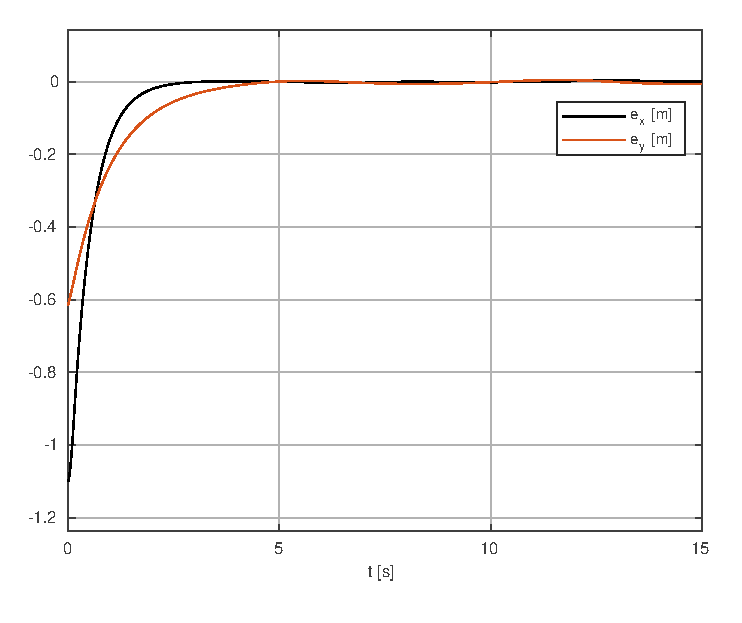
\includegraphics[width=0.5\linewidth]{lin/feedback/e.eps}	
\caption{Wyniki symulacji dla zadania śledzenia trajektorii zmiennej w czasie: a) wykres konfiguracji $q$ oraz konfiguracji zadanej $q_d$, b) prędkości $u$ oraz prędkości zadanych $u_d$, c) ruchu pojazdu, d) uchybów $e$. Przyjęto parametry $L_Z=0.5[m]$ oraz $\beta_Z=0.3[\degree]$. Dobrano macierz wzmocnień $K$=\texttt{diag}$(2.0; 1.0)$. }\end{figure}
\begin{figure}[H]
	a)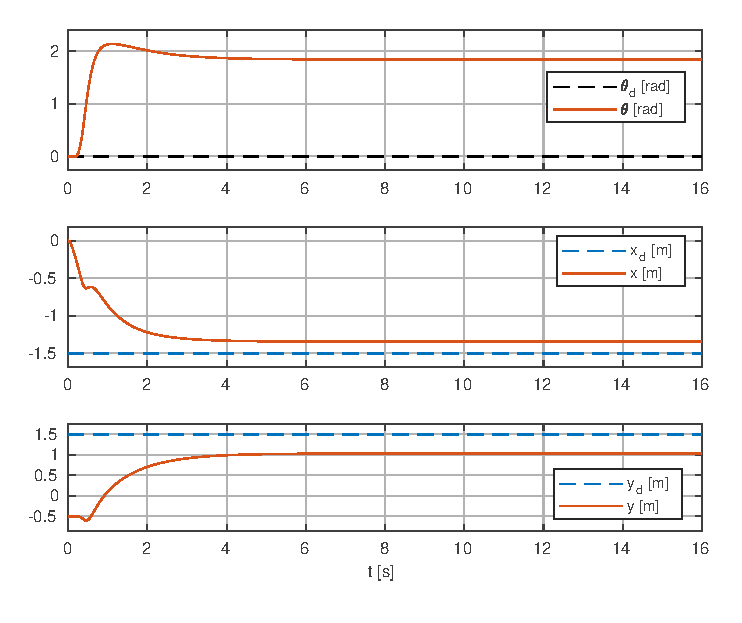
\includegraphics[width=0.5\linewidth]{lin/feedback/q_ps.eps}
	b)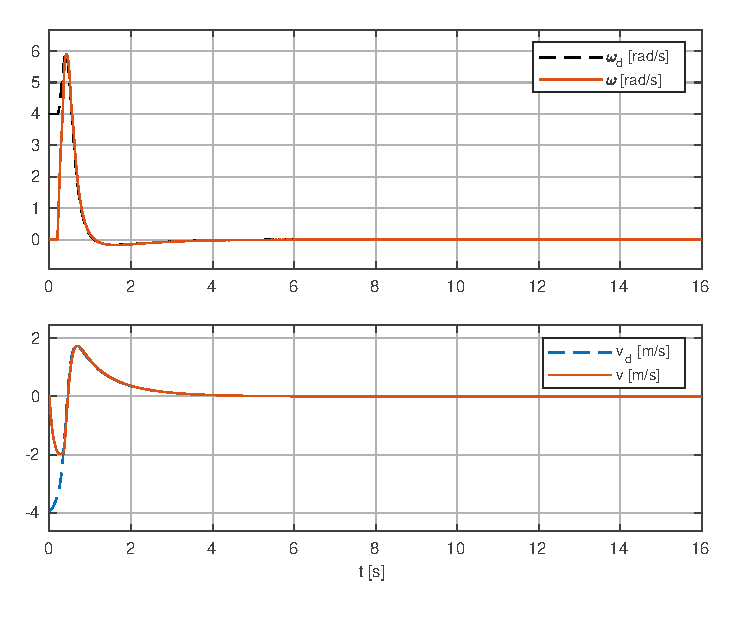
\includegraphics[width=0.5\linewidth]{lin/feedback/u_ps.eps}\\
	c)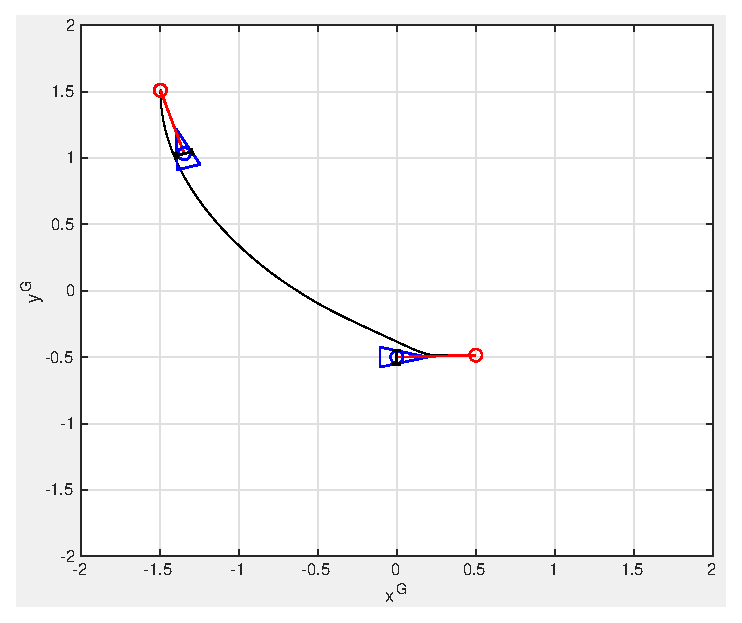
\includegraphics[width=0.5\linewidth]{lin/feedback/cartplot_ps.eps}	
	d)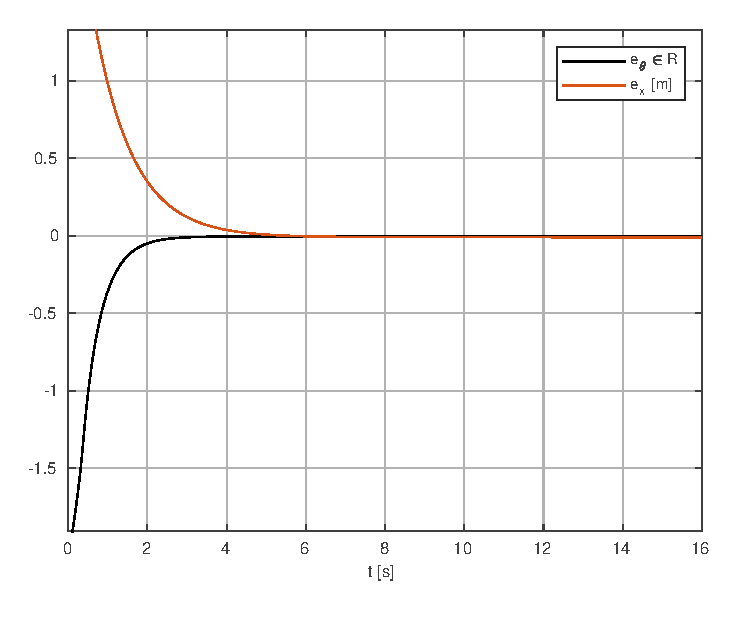
\includegraphics[width=0.5\linewidth]{lin/feedback/e_ps.eps}	
	\caption{Wyniki symulacji dla zadania sterowania do punktu, $L_Z=0.5[m]$ oraz $\beta_Z=0.3[\degree]$. Dobrano macierz wzmocnień $K$=\texttt{diag}$(2.0; 1.0)$. }\end{figure}

\begin{figure}[H]
\subsubsection{Algorytm dla zadania śledzenia trajektorii zadanej}
Przyjęto równanie z syntezą sterownika (4.35$\div$4.36):
$$
 k_{11} = k_{22} = -2\zeta\sqrt{u_{d1}^2+\alpha u_{d2}^2}, \quad k_{13}=-\alpha u_{d2}
$$
	a)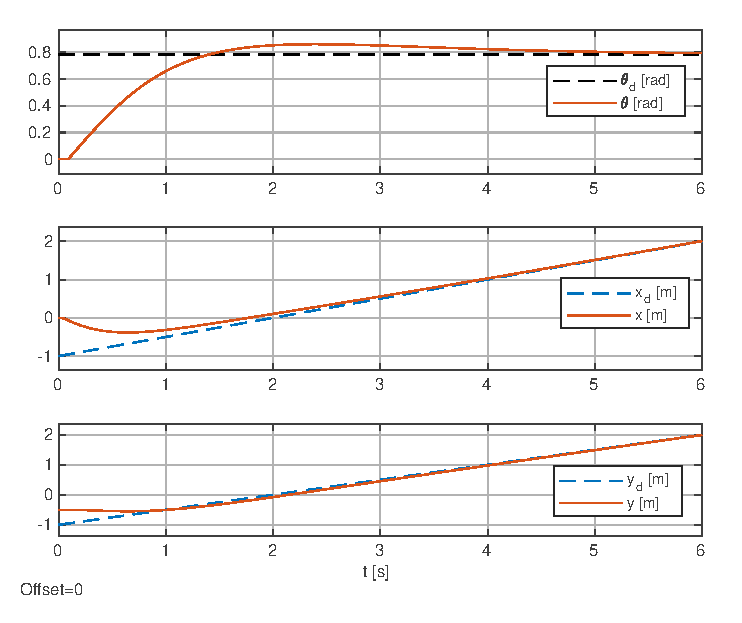
\includegraphics[width=0.5\linewidth]{lin/approx/q_tt.eps}
	b)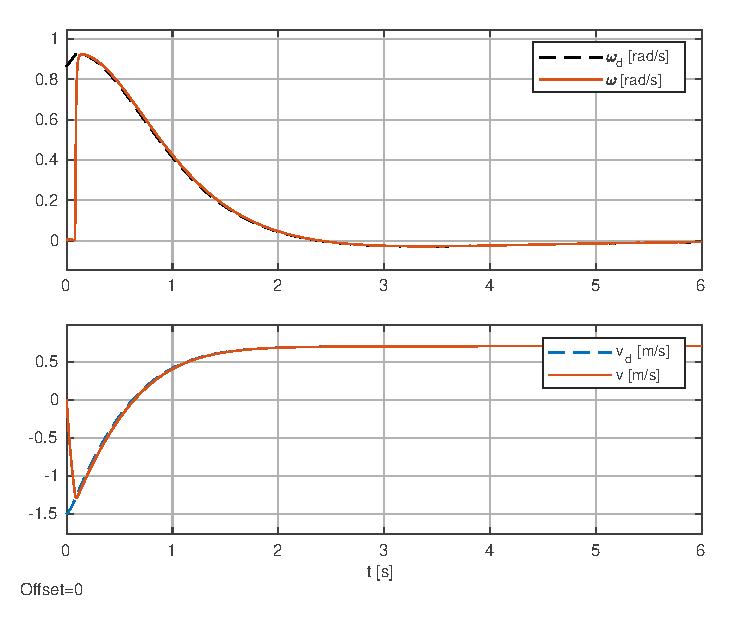
\includegraphics[width=0.5\linewidth]{lin/approx/u_tt.eps}\\
	c)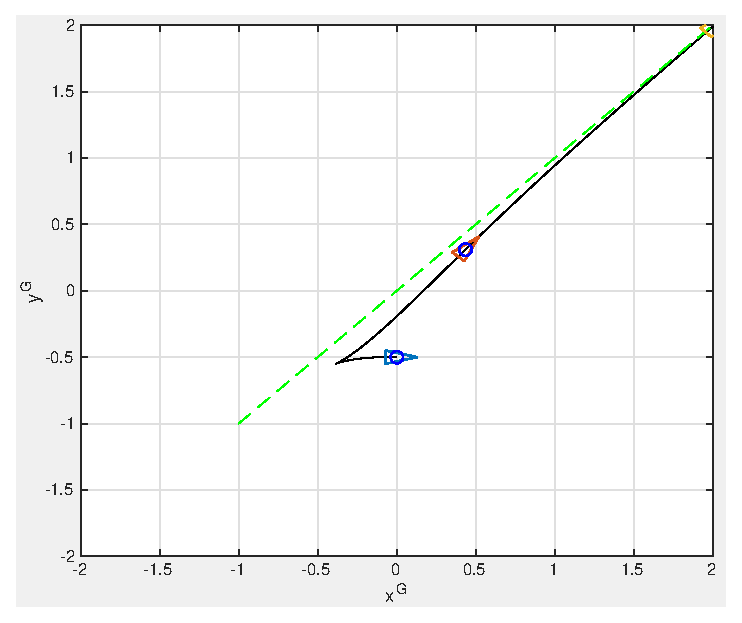
\includegraphics[width=0.5\linewidth]{lin/approx/cartplot_tt}	
	d)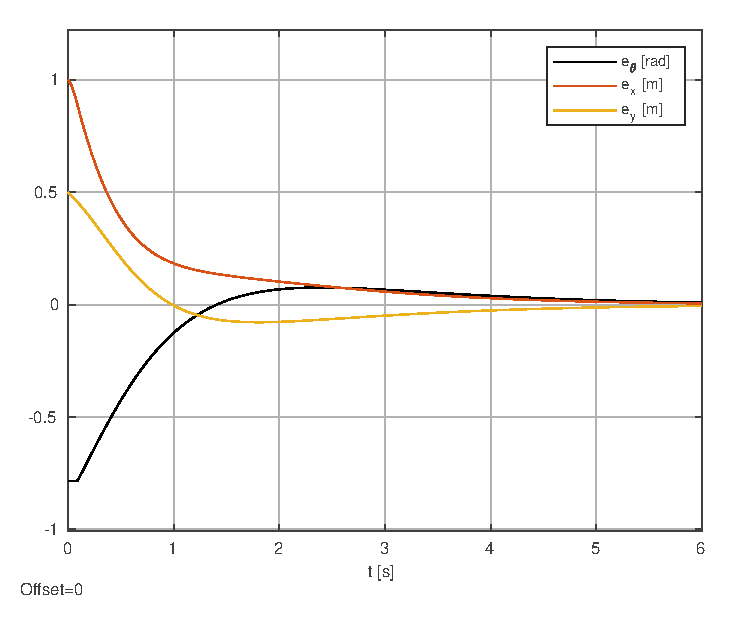
\includegraphics[width=0.5\linewidth]{lin/approx/e_tt.eps}
\caption{Wyniki symulacji dla zadania śledzenia trajektorii zadanej:  a) wykres konfiguracji $q$ oraz konfiguracji zadanej $q_d$, b) prędkości $u$ oraz prędkości zadanych $u_d$, c) ruchu pojazdu, d) uchybów $e$. Przyjęto wartości współczynników $\zeta=1, \quad \alpha=2$.}\end{figure}


\begin{figure}[H]
\subsubsection{Algorytm dla zadania podążania wzdłuż ścieżki}
Przyjęto postać sterownika (4.59) wraz z syntezą parametryczną (4.62$\div$4.63):
$$
u_1 = u + \frac{u_2\kappa_d(S)cos(e_\theta)}{1-e_l\kappa_d(S)}, \quad k_1=\omega_n^2,\quad k_2=2\zeta\omega_n
$$
	a)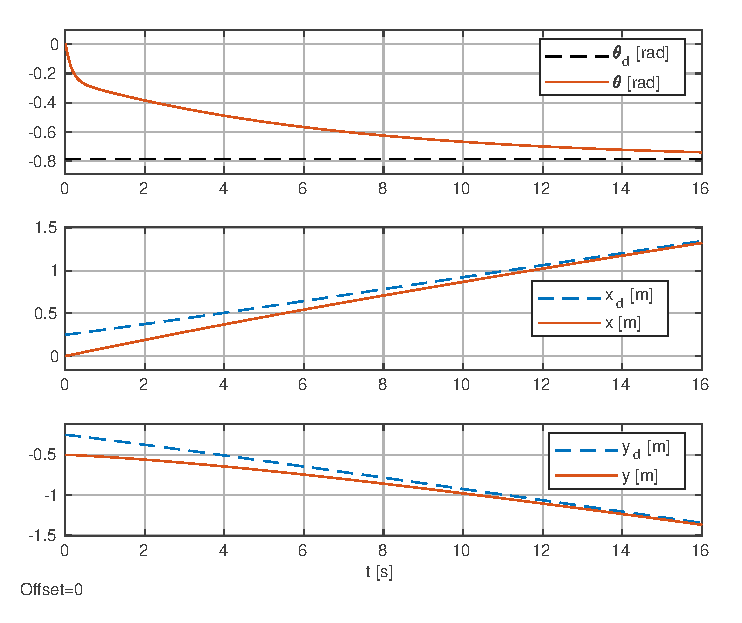
\includegraphics[width=0.5\linewidth]{lin/approx/q_pf.eps}
	b)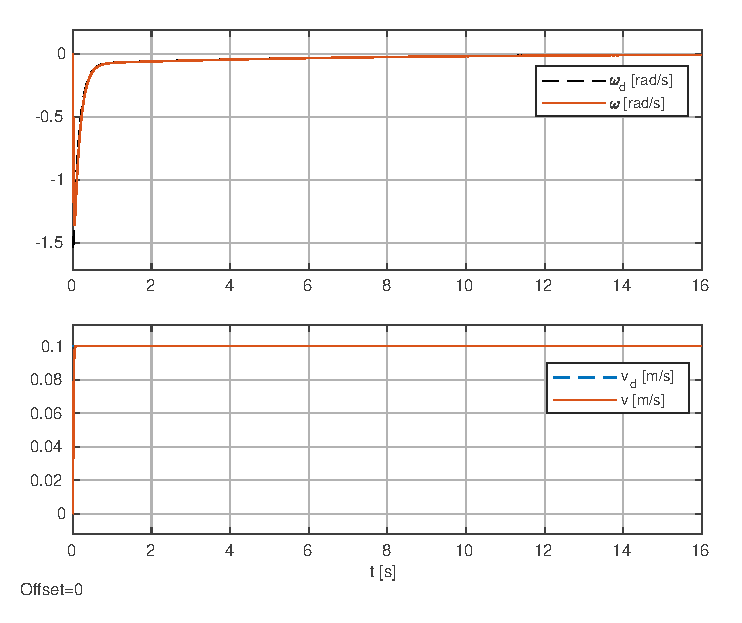
\includegraphics[width=0.5\linewidth]{lin/approx/u_pf.eps}\\
	c)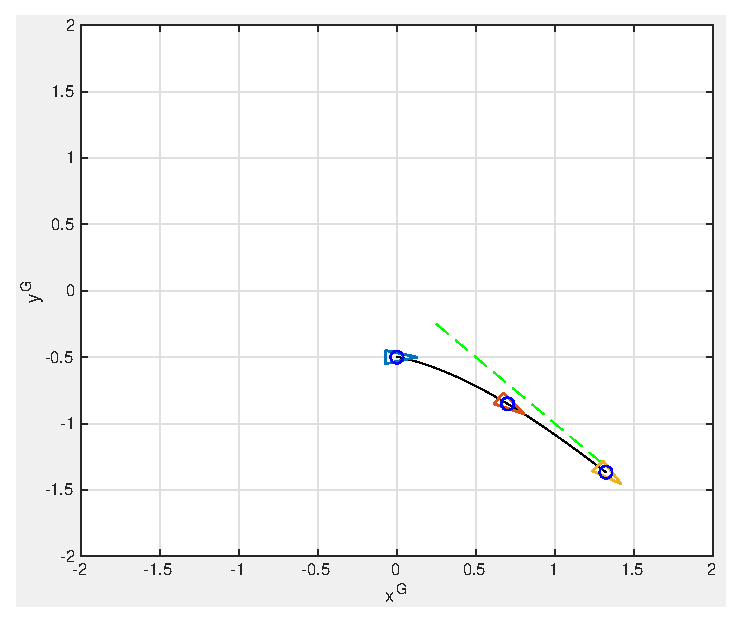
\includegraphics[width=0.5\linewidth]{lin/approx/cartplot_pf}	
	d)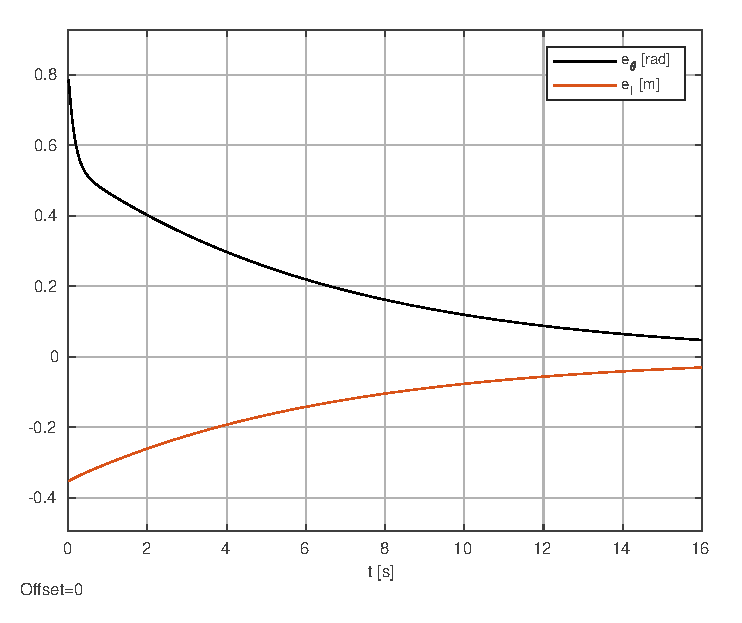
\includegraphics[width=0.5\linewidth]{lin/approx/e_pf.eps}
	\caption{Wyniki symulacji dla zadania podążania wzdłuż ścieżki:  a) wykres konfiguracji $q$ oraz konfiguracji zadanej $q_d$, b) prędkości $u$ oraz prędkości zadanych $u_d$, c) ruchu pojazdu, d) uchybów $e$. Przyjęto wartości współczynników $\zeta=1, \quad \omega_n=3, \quad k_1 = 9, \quad k_2 = 6$.}\end{figure}


\begin{figure}[H]
\subsection{Ciągły stabilizator Pometa jawnie zależny od czasu}\label{pomet_ps}
Do algorytmu sterowania wykorzystano funkcję $h$ postaci (5.36):
$$
h(t,\tilde{e}) = k_4\frac{\tilde{e}_2^2+\tilde{e}_3^2}{\tilde{e}_2^2+\tilde{e}_3^2+\delta_p}\cos(\Omega t)
$$
	a)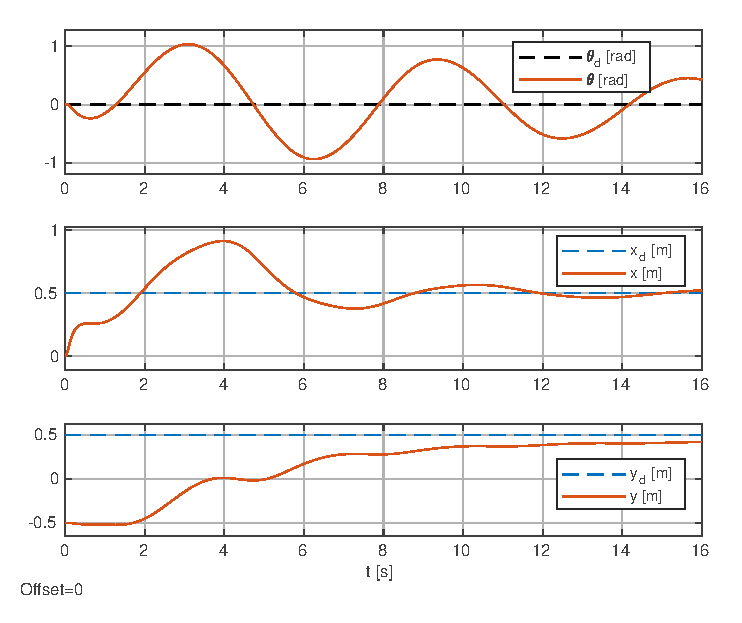
\includegraphics[width=0.5\linewidth]{pomet/q.eps}
	b)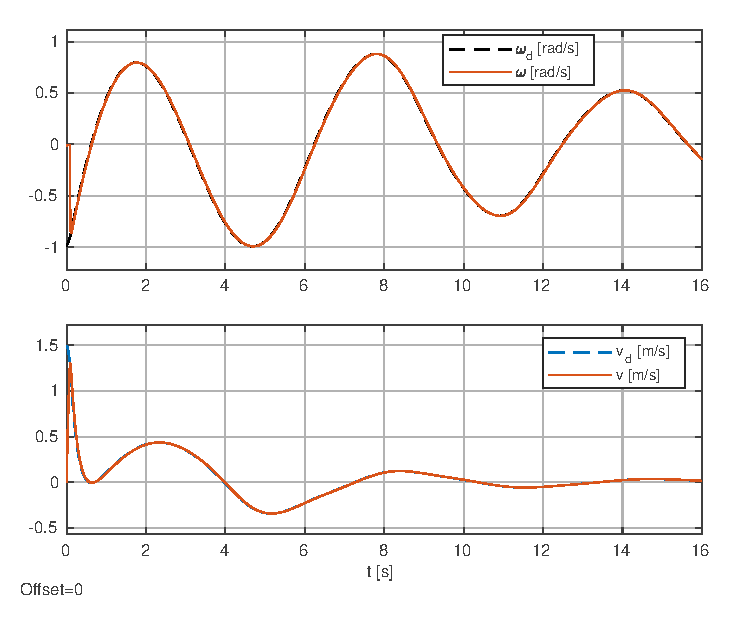
\includegraphics[width=0.5\linewidth]{pomet/u.eps}\\
	c)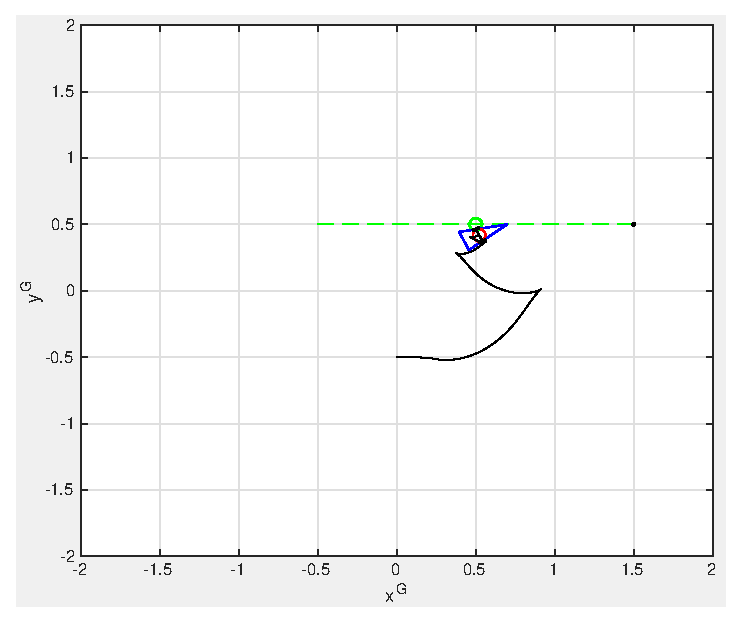
\includegraphics[width=0.5\linewidth]{pomet/cartplot.eps}	
	d)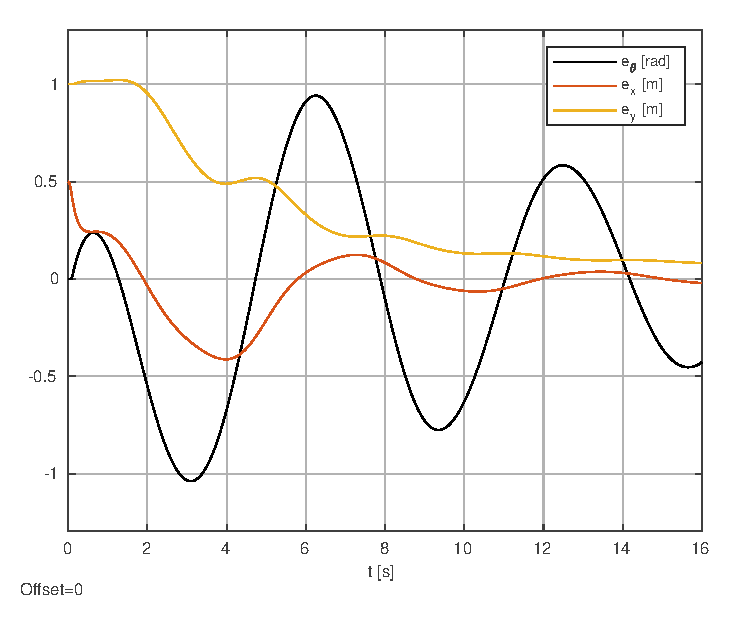
\includegraphics[width=0.5\linewidth]{pomet/e.eps}
	\caption{Wyniki symulacji dla zadania podążania do punktu: a) wykres konfiguracji $q$ oraz konfiguracji zadanej $q_d$, b) prędkości $u$ oraz prędkości zadanych $u_d$, c) ruchu pojazdu, d) uchybów $e$. Wartości przyjętych współczynników $k_1=k_2=k_3=k_4=1, \quad \delta_p=0.01, \quad \Omega=1$.}\end{figure}
\subsection{Sterowniki nieciągłe metody VFO}

\begin{figure}[H]
\subsubsection{Algorytm VFO dla zadania śledzenia trajektorii}\label{vfo_tt}
	a)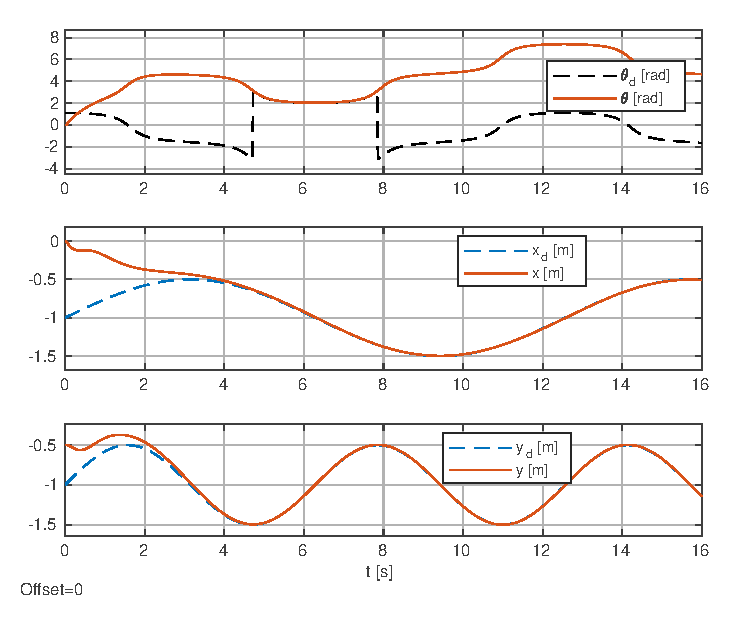
\includegraphics[width=0.5\linewidth]{vfo/q_tt.eps}
	b)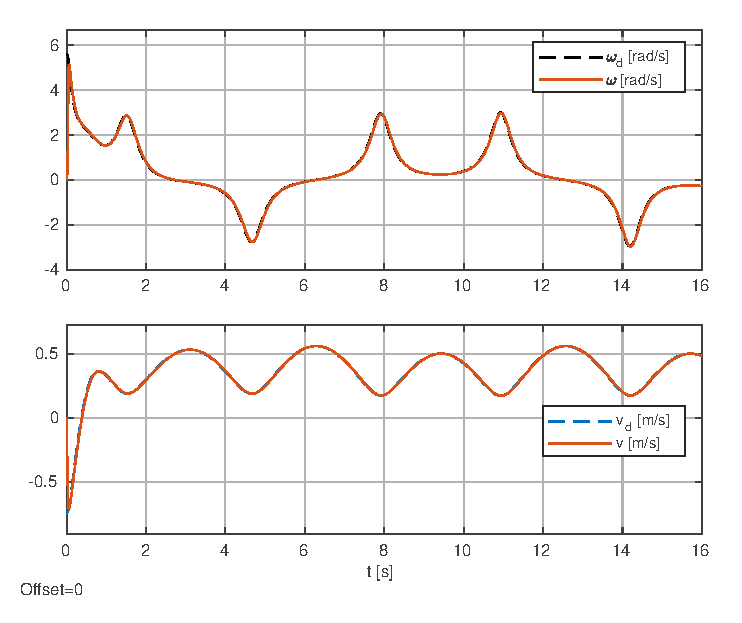
\includegraphics[width=0.5\linewidth]{vfo/u_tt.eps}\\
	c)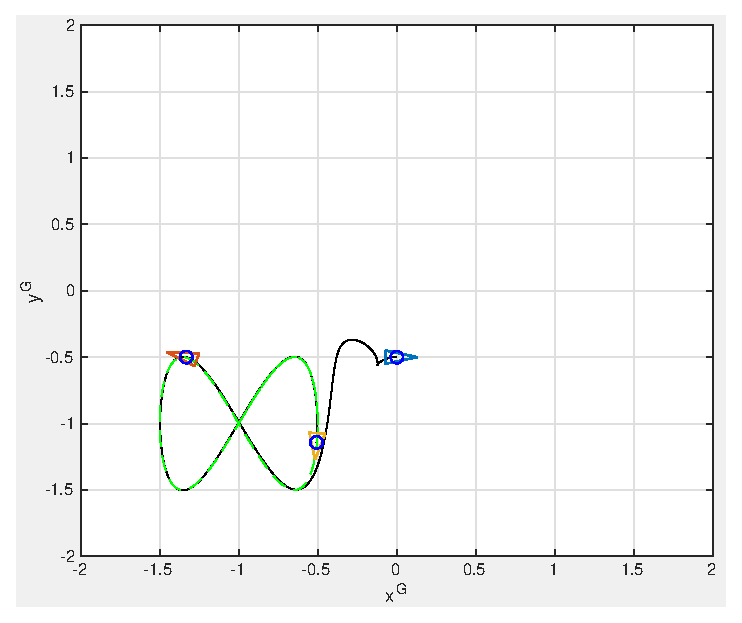
\includegraphics[width=0.5\linewidth]{vfo/cartplot_tt.eps}	
	d)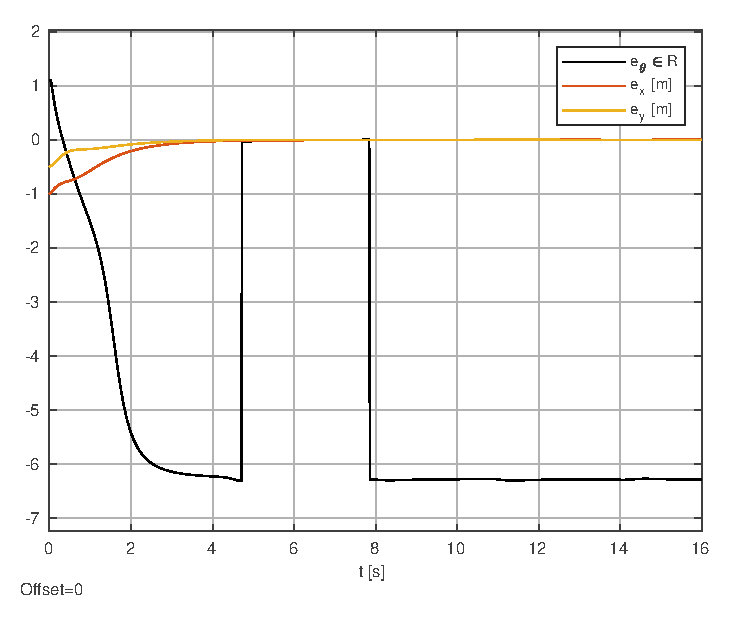
\includegraphics[width=0.5\linewidth]{vfo/e_tt.eps}
	\caption{Wyniki symulacji dla zadania śledzenia trajektorii: a) wykres konfiguracji $q$ oraz konfiguracji zadanej $q_d$, b) prędkości $u$ oraz prędkości zadanych $u_d$, c) ruchu pojazdu, d) uchybów $e$. Wartości przyjętych współczynników $\zeta_d=1,\quad k_p =1, \quad \eta=0.8k_p,\quad \delta=0.001,\quad k_a=2k_p$.}\end{figure}

\begin{figure}[H]
	\subsubsection{Algorytm VFO dla zadania podążania do punktu}\label{vfo_ps}
	a)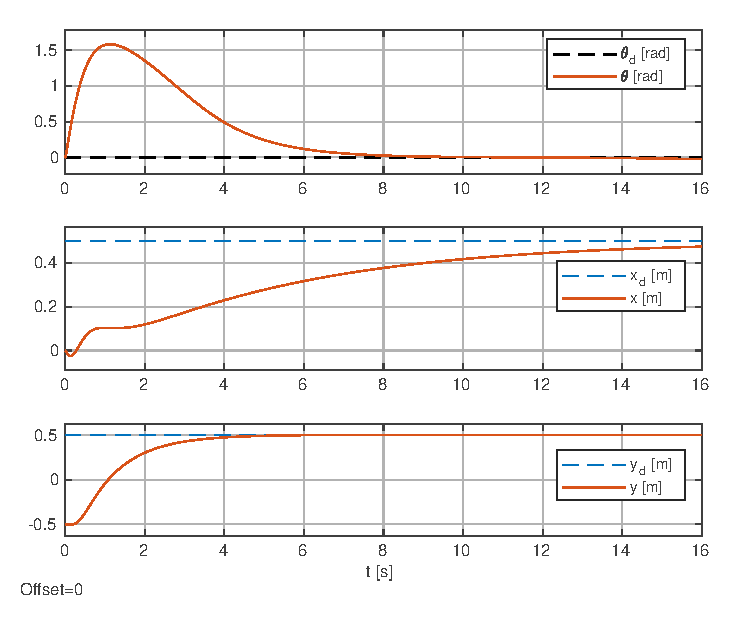
\includegraphics[width=0.5\linewidth]{vfo/q_ps.eps}
	b)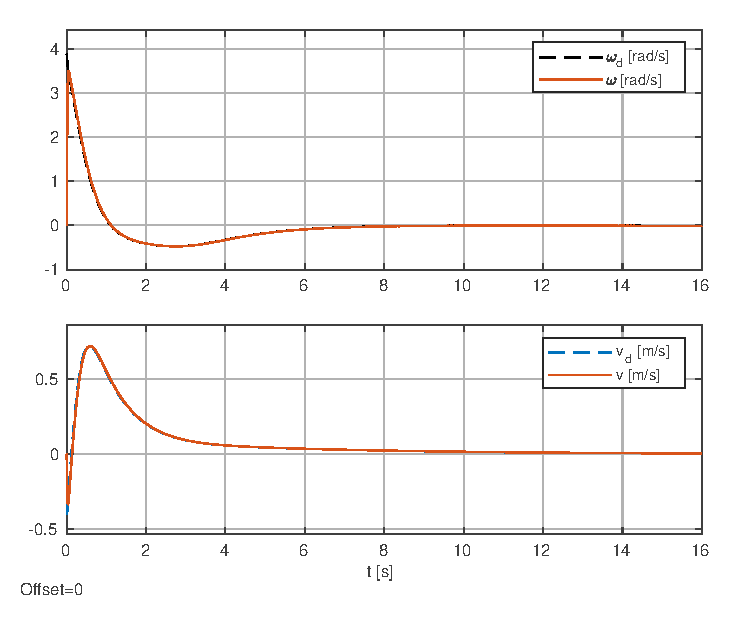
\includegraphics[width=0.5\linewidth]{vfo/u_ps.eps}\\
	c)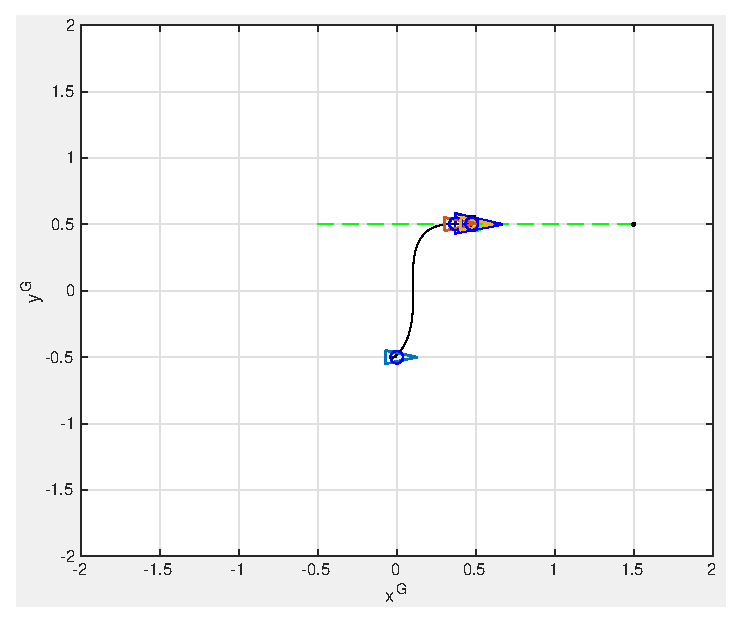
\includegraphics[width=0.5\linewidth]{vfo/cartplot_ps.eps}	
	d)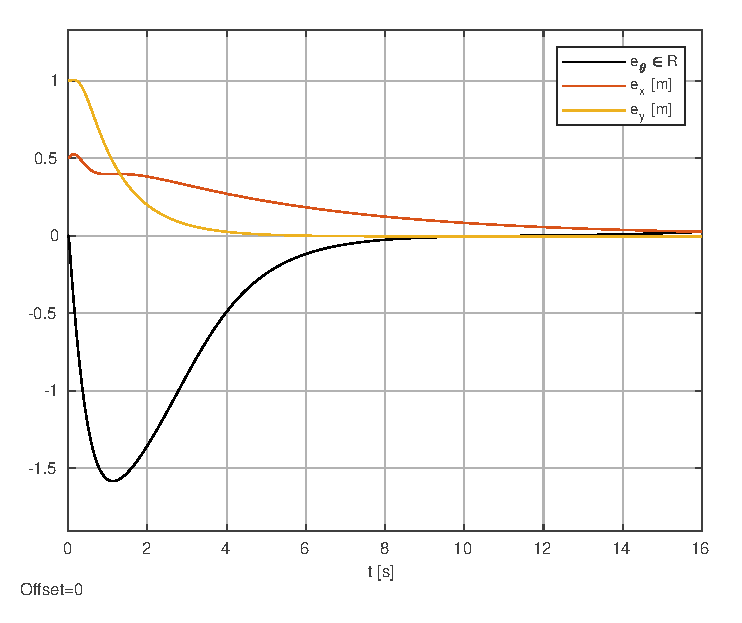
\includegraphics[width=0.5\linewidth]{vfo/e_ps.eps}
	\caption{Wyniki symulacji dla zadania podążania do punktu: a) wykres konfiguracji $q$ oraz konfiguracji zadanej $q_d$, b) prędkości $u$ oraz prędkości zadanych $u_d$, c) ruchu pojazdu, d) uchybów $e$. Wartości przyjętych współczynników $\zeta_d=1,\quad k_p =1, \quad \eta=0.8k_p,\quad \delta=0.001,\quad k_a=2k_p$.}\end{figure}


\newpage\section{Analiza wyników}
Poniżej przedstawiono odpowiedzi w zależności od zadania ruchu.
\subsection{Zadanie podążania do punktu}\label{analiza_ps}
Kryterium oceny zostało wybrane jako czas ustalenia się odpowiedzi do tunelu ok. 10\% maksymalnej wartości $e_\theta$.

\noindent\begin{table}[h]\caption{Porównanie czasu ustalenia uchybu $e_\theta$ dla zadania sterowania do punktu}
\begin{tabularx}{\textwidth} { 
		| >{\centering\arraybackslash}X 
		| >{\centering\arraybackslash}X 
		| >{\centering\arraybackslash}X 
		| >{\centering\arraybackslash}X |}
	\hline
	  & VFO (\ref{vfo_ps}) & Pomet (\ref{pomet_ps}) \\
	\hline
	$T_{ust}$ [s]  & 7  & >16  \\
	\hline
\end{tabularx}
\end{table}

\subsection{Zadanie śledzenia trajektorii}\label{analiza_tt}
Do porównania wybrano trajektorię ósemkową.
\noindent\begin{table}[h]\caption{Porównanie czasu ustalenia uchybów $e_x$, $e_y$ dla zadania podążania wzdłuż trajektorii ósemkowej}
	\begin{tabularx}{\textwidth} { 
			| >{\centering\arraybackslash}X 
			| >{\centering\arraybackslash}X 
			| >{\centering\arraybackslash}X 
			| >{\centering\arraybackslash}X |}
		\hline
		& VFO (\ref{vfo_tt}) & Linearyzacja (\ref{linear_tt}) \\
		\hline
		$T_{ust}$ [s]  & 3  & 1  \\
		\hline
	\end{tabularx}
\end{table}

\section{Wnioski}
Porównując możliwości sterowników w kwestii odtwarzania trajektorii zadanej, najbardziej wszechstronnym wyborem zdaje się być sterownik VFO. Umożliwia on odtworzenie każdej ścieżki, bez konieczności wyprowadzania np. punktu Z, jak dla sterownika wynikającego z metody linearyzacji sprzężeniem zwrotnym. 

W przypadku zadania sterowania do punktu, korzystna jest synteza sterowników VFO, dającego szybszą zbieżność do zadanego punktu (porównanie w rozdziale \ref{analiza_ps}) oraz Pometa, gwarantującego odtworzenia zadanego kąta $\theta_d$. Połączenie sterowników umożliwi wjazd do wnęki, pozwoli na parkowanie równoległe.

Sterowniki wynikające z metod linearyzacji, mimo ich ograniczeń i prostoty implementacji, przynoszą satysfakcjonujące rezultaty, co ukazują wykresy uchybów oraz porównanie wyników w rozdziale \ref{analiza_tt}. Pozwalają odtworzyć zadane trajektorie, lecz z istotnymi ograniczeniami - m.in. punktem Z.

Generator trajektorii parametryzowanej czasem $t$ umożliwia odtworzenie każdej z krzywych zadanych. Jest to najbardziej wszechstronna możliwość. Jednakże znacznym ograniczeniem jest pobudzanie modelu robota tylko i wyłącznie czasem, niezależnym od konfiguracji. W niektórych implementacjach jest to poważne ograniczenie.

Zastosowany regulator PI dla pętli podrzędnej umożliwia zminimalizowanie efektów oporu wynikających z dynamiki robota mobilnego, pozwalając na implementację sterownika pętli nadrzędnej, generującego zadane prędkości $u_d$.







\end{document}
